
% Default to the notebook output style

    


% Inherit from the specified cell style.




    
\documentclass[11pt]{article}

    
    
    \usepackage[T1]{fontenc}
    % Nicer default font (+ math font) than Computer Modern for most use cases
    \usepackage{mathpazo}

    % Basic figure setup, for now with no caption control since it's done
    % automatically by Pandoc (which extracts ![](path) syntax from Markdown).
    \usepackage{graphicx}
    % We will generate all images so they have a width \maxwidth. This means
    % that they will get their normal width if they fit onto the page, but
    % are scaled down if they would overflow the margins.
    \makeatletter
    \def\maxwidth{\ifdim\Gin@nat@width>\linewidth\linewidth
    \else\Gin@nat@width\fi}
    \makeatother
    \let\Oldincludegraphics\includegraphics
    % Set max figure width to be 80% of text width, for now hardcoded.
    \renewcommand{\includegraphics}[1]{\Oldincludegraphics[width=.8\maxwidth]{#1}}
    % Ensure that by default, figures have no caption (until we provide a
    % proper Figure object with a Caption API and a way to capture that
    % in the conversion process - todo).
    \usepackage{caption}
    \DeclareCaptionLabelFormat{nolabel}{}
    \captionsetup{labelformat=nolabel}

    \usepackage{adjustbox} % Used to constrain images to a maximum size 
    \usepackage{xcolor} % Allow colors to be defined
    \usepackage{enumerate} % Needed for markdown enumerations to work
    \usepackage{geometry} % Used to adjust the document margins
    \usepackage{amsmath} % Equations
    \usepackage{amssymb} % Equations
    \usepackage{textcomp} % defines textquotesingle
    % Hack from http://tex.stackexchange.com/a/47451/13684:
    \AtBeginDocument{%
        \def\PYZsq{\textquotesingle}% Upright quotes in Pygmentized code
    }
    \usepackage{upquote} % Upright quotes for verbatim code
    \usepackage{eurosym} % defines \euro
    \usepackage[mathletters]{ucs} % Extended unicode (utf-8) support
    \usepackage[utf8x]{inputenc} % Allow utf-8 characters in the tex document
    \usepackage{fancyvrb} % verbatim replacement that allows latex
    \usepackage{grffile} % extends the file name processing of package graphics 
                         % to support a larger range 
    % The hyperref package gives us a pdf with properly built
    % internal navigation ('pdf bookmarks' for the table of contents,
    % internal cross-reference links, web links for URLs, etc.)
    \usepackage{hyperref}
    \usepackage{longtable} % longtable support required by pandoc >1.10
    \usepackage{booktabs}  % table support for pandoc > 1.12.2
    \usepackage[inline]{enumitem} % IRkernel/repr support (it uses the enumerate* environment)
    \usepackage[normalem]{ulem} % ulem is needed to support strikethroughs (\sout)
                                % normalem makes italics be italics, not underlines
    

    
    
    % Colors for the hyperref package
    \definecolor{urlcolor}{rgb}{0,.145,.698}
    \definecolor{linkcolor}{rgb}{.71,0.21,0.01}
    \definecolor{citecolor}{rgb}{.12,.54,.11}

    % ANSI colors
    \definecolor{ansi-black}{HTML}{3E424D}
    \definecolor{ansi-black-intense}{HTML}{282C36}
    \definecolor{ansi-red}{HTML}{E75C58}
    \definecolor{ansi-red-intense}{HTML}{B22B31}
    \definecolor{ansi-green}{HTML}{00A250}
    \definecolor{ansi-green-intense}{HTML}{007427}
    \definecolor{ansi-yellow}{HTML}{DDB62B}
    \definecolor{ansi-yellow-intense}{HTML}{B27D12}
    \definecolor{ansi-blue}{HTML}{208FFB}
    \definecolor{ansi-blue-intense}{HTML}{0065CA}
    \definecolor{ansi-magenta}{HTML}{D160C4}
    \definecolor{ansi-magenta-intense}{HTML}{A03196}
    \definecolor{ansi-cyan}{HTML}{60C6C8}
    \definecolor{ansi-cyan-intense}{HTML}{258F8F}
    \definecolor{ansi-white}{HTML}{C5C1B4}
    \definecolor{ansi-white-intense}{HTML}{A1A6B2}

    % commands and environments needed by pandoc snippets
    % extracted from the output of `pandoc -s`
    \providecommand{\tightlist}{%
      \setlength{\itemsep}{0pt}\setlength{\parskip}{0pt}}
    \DefineVerbatimEnvironment{Highlighting}{Verbatim}{commandchars=\\\{\}}
    % Add ',fontsize=\small' for more characters per line
    \newenvironment{Shaded}{}{}
    \newcommand{\KeywordTok}[1]{\textcolor[rgb]{0.00,0.44,0.13}{\textbf{{#1}}}}
    \newcommand{\DataTypeTok}[1]{\textcolor[rgb]{0.56,0.13,0.00}{{#1}}}
    \newcommand{\DecValTok}[1]{\textcolor[rgb]{0.25,0.63,0.44}{{#1}}}
    \newcommand{\BaseNTok}[1]{\textcolor[rgb]{0.25,0.63,0.44}{{#1}}}
    \newcommand{\FloatTok}[1]{\textcolor[rgb]{0.25,0.63,0.44}{{#1}}}
    \newcommand{\CharTok}[1]{\textcolor[rgb]{0.25,0.44,0.63}{{#1}}}
    \newcommand{\StringTok}[1]{\textcolor[rgb]{0.25,0.44,0.63}{{#1}}}
    \newcommand{\CommentTok}[1]{\textcolor[rgb]{0.38,0.63,0.69}{\textit{{#1}}}}
    \newcommand{\OtherTok}[1]{\textcolor[rgb]{0.00,0.44,0.13}{{#1}}}
    \newcommand{\AlertTok}[1]{\textcolor[rgb]{1.00,0.00,0.00}{\textbf{{#1}}}}
    \newcommand{\FunctionTok}[1]{\textcolor[rgb]{0.02,0.16,0.49}{{#1}}}
    \newcommand{\RegionMarkerTok}[1]{{#1}}
    \newcommand{\ErrorTok}[1]{\textcolor[rgb]{1.00,0.00,0.00}{\textbf{{#1}}}}
    \newcommand{\NormalTok}[1]{{#1}}
    
    % Additional commands for more recent versions of Pandoc
    \newcommand{\ConstantTok}[1]{\textcolor[rgb]{0.53,0.00,0.00}{{#1}}}
    \newcommand{\SpecialCharTok}[1]{\textcolor[rgb]{0.25,0.44,0.63}{{#1}}}
    \newcommand{\VerbatimStringTok}[1]{\textcolor[rgb]{0.25,0.44,0.63}{{#1}}}
    \newcommand{\SpecialStringTok}[1]{\textcolor[rgb]{0.73,0.40,0.53}{{#1}}}
    \newcommand{\ImportTok}[1]{{#1}}
    \newcommand{\DocumentationTok}[1]{\textcolor[rgb]{0.73,0.13,0.13}{\textit{{#1}}}}
    \newcommand{\AnnotationTok}[1]{\textcolor[rgb]{0.38,0.63,0.69}{\textbf{\textit{{#1}}}}}
    \newcommand{\CommentVarTok}[1]{\textcolor[rgb]{0.38,0.63,0.69}{\textbf{\textit{{#1}}}}}
    \newcommand{\VariableTok}[1]{\textcolor[rgb]{0.10,0.09,0.49}{{#1}}}
    \newcommand{\ControlFlowTok}[1]{\textcolor[rgb]{0.00,0.44,0.13}{\textbf{{#1}}}}
    \newcommand{\OperatorTok}[1]{\textcolor[rgb]{0.40,0.40,0.40}{{#1}}}
    \newcommand{\BuiltInTok}[1]{{#1}}
    \newcommand{\ExtensionTok}[1]{{#1}}
    \newcommand{\PreprocessorTok}[1]{\textcolor[rgb]{0.74,0.48,0.00}{{#1}}}
    \newcommand{\AttributeTok}[1]{\textcolor[rgb]{0.49,0.56,0.16}{{#1}}}
    \newcommand{\InformationTok}[1]{\textcolor[rgb]{0.38,0.63,0.69}{\textbf{\textit{{#1}}}}}
    \newcommand{\WarningTok}[1]{\textcolor[rgb]{0.38,0.63,0.69}{\textbf{\textit{{#1}}}}}
    
    
    % Define a nice break command that doesn't care if a line doesn't already
    % exist.
    \def\br{\hspace*{\fill} \\* }
    % Math Jax compatability definitions
    \def\gt{>}
    \def\lt{<}
    % Document parameters
    \title{norheim\_final\_project}
    
    
    

    % Pygments definitions
    
\makeatletter
\def\PY@reset{\let\PY@it=\relax \let\PY@bf=\relax%
    \let\PY@ul=\relax \let\PY@tc=\relax%
    \let\PY@bc=\relax \let\PY@ff=\relax}
\def\PY@tok#1{\csname PY@tok@#1\endcsname}
\def\PY@toks#1+{\ifx\relax#1\empty\else%
    \PY@tok{#1}\expandafter\PY@toks\fi}
\def\PY@do#1{\PY@bc{\PY@tc{\PY@ul{%
    \PY@it{\PY@bf{\PY@ff{#1}}}}}}}
\def\PY#1#2{\PY@reset\PY@toks#1+\relax+\PY@do{#2}}

\expandafter\def\csname PY@tok@gd\endcsname{\def\PY@tc##1{\textcolor[rgb]{0.63,0.00,0.00}{##1}}}
\expandafter\def\csname PY@tok@gu\endcsname{\let\PY@bf=\textbf\def\PY@tc##1{\textcolor[rgb]{0.50,0.00,0.50}{##1}}}
\expandafter\def\csname PY@tok@gt\endcsname{\def\PY@tc##1{\textcolor[rgb]{0.00,0.27,0.87}{##1}}}
\expandafter\def\csname PY@tok@gs\endcsname{\let\PY@bf=\textbf}
\expandafter\def\csname PY@tok@gr\endcsname{\def\PY@tc##1{\textcolor[rgb]{1.00,0.00,0.00}{##1}}}
\expandafter\def\csname PY@tok@cm\endcsname{\let\PY@it=\textit\def\PY@tc##1{\textcolor[rgb]{0.25,0.50,0.50}{##1}}}
\expandafter\def\csname PY@tok@vg\endcsname{\def\PY@tc##1{\textcolor[rgb]{0.10,0.09,0.49}{##1}}}
\expandafter\def\csname PY@tok@vi\endcsname{\def\PY@tc##1{\textcolor[rgb]{0.10,0.09,0.49}{##1}}}
\expandafter\def\csname PY@tok@vm\endcsname{\def\PY@tc##1{\textcolor[rgb]{0.10,0.09,0.49}{##1}}}
\expandafter\def\csname PY@tok@mh\endcsname{\def\PY@tc##1{\textcolor[rgb]{0.40,0.40,0.40}{##1}}}
\expandafter\def\csname PY@tok@cs\endcsname{\let\PY@it=\textit\def\PY@tc##1{\textcolor[rgb]{0.25,0.50,0.50}{##1}}}
\expandafter\def\csname PY@tok@ge\endcsname{\let\PY@it=\textit}
\expandafter\def\csname PY@tok@vc\endcsname{\def\PY@tc##1{\textcolor[rgb]{0.10,0.09,0.49}{##1}}}
\expandafter\def\csname PY@tok@il\endcsname{\def\PY@tc##1{\textcolor[rgb]{0.40,0.40,0.40}{##1}}}
\expandafter\def\csname PY@tok@go\endcsname{\def\PY@tc##1{\textcolor[rgb]{0.53,0.53,0.53}{##1}}}
\expandafter\def\csname PY@tok@cp\endcsname{\def\PY@tc##1{\textcolor[rgb]{0.74,0.48,0.00}{##1}}}
\expandafter\def\csname PY@tok@gi\endcsname{\def\PY@tc##1{\textcolor[rgb]{0.00,0.63,0.00}{##1}}}
\expandafter\def\csname PY@tok@gh\endcsname{\let\PY@bf=\textbf\def\PY@tc##1{\textcolor[rgb]{0.00,0.00,0.50}{##1}}}
\expandafter\def\csname PY@tok@ni\endcsname{\let\PY@bf=\textbf\def\PY@tc##1{\textcolor[rgb]{0.60,0.60,0.60}{##1}}}
\expandafter\def\csname PY@tok@nl\endcsname{\def\PY@tc##1{\textcolor[rgb]{0.63,0.63,0.00}{##1}}}
\expandafter\def\csname PY@tok@nn\endcsname{\let\PY@bf=\textbf\def\PY@tc##1{\textcolor[rgb]{0.00,0.00,1.00}{##1}}}
\expandafter\def\csname PY@tok@no\endcsname{\def\PY@tc##1{\textcolor[rgb]{0.53,0.00,0.00}{##1}}}
\expandafter\def\csname PY@tok@na\endcsname{\def\PY@tc##1{\textcolor[rgb]{0.49,0.56,0.16}{##1}}}
\expandafter\def\csname PY@tok@nb\endcsname{\def\PY@tc##1{\textcolor[rgb]{0.00,0.50,0.00}{##1}}}
\expandafter\def\csname PY@tok@nc\endcsname{\let\PY@bf=\textbf\def\PY@tc##1{\textcolor[rgb]{0.00,0.00,1.00}{##1}}}
\expandafter\def\csname PY@tok@nd\endcsname{\def\PY@tc##1{\textcolor[rgb]{0.67,0.13,1.00}{##1}}}
\expandafter\def\csname PY@tok@ne\endcsname{\let\PY@bf=\textbf\def\PY@tc##1{\textcolor[rgb]{0.82,0.25,0.23}{##1}}}
\expandafter\def\csname PY@tok@nf\endcsname{\def\PY@tc##1{\textcolor[rgb]{0.00,0.00,1.00}{##1}}}
\expandafter\def\csname PY@tok@si\endcsname{\let\PY@bf=\textbf\def\PY@tc##1{\textcolor[rgb]{0.73,0.40,0.53}{##1}}}
\expandafter\def\csname PY@tok@s2\endcsname{\def\PY@tc##1{\textcolor[rgb]{0.73,0.13,0.13}{##1}}}
\expandafter\def\csname PY@tok@nt\endcsname{\let\PY@bf=\textbf\def\PY@tc##1{\textcolor[rgb]{0.00,0.50,0.00}{##1}}}
\expandafter\def\csname PY@tok@nv\endcsname{\def\PY@tc##1{\textcolor[rgb]{0.10,0.09,0.49}{##1}}}
\expandafter\def\csname PY@tok@s1\endcsname{\def\PY@tc##1{\textcolor[rgb]{0.73,0.13,0.13}{##1}}}
\expandafter\def\csname PY@tok@dl\endcsname{\def\PY@tc##1{\textcolor[rgb]{0.73,0.13,0.13}{##1}}}
\expandafter\def\csname PY@tok@ch\endcsname{\let\PY@it=\textit\def\PY@tc##1{\textcolor[rgb]{0.25,0.50,0.50}{##1}}}
\expandafter\def\csname PY@tok@m\endcsname{\def\PY@tc##1{\textcolor[rgb]{0.40,0.40,0.40}{##1}}}
\expandafter\def\csname PY@tok@gp\endcsname{\let\PY@bf=\textbf\def\PY@tc##1{\textcolor[rgb]{0.00,0.00,0.50}{##1}}}
\expandafter\def\csname PY@tok@sh\endcsname{\def\PY@tc##1{\textcolor[rgb]{0.73,0.13,0.13}{##1}}}
\expandafter\def\csname PY@tok@ow\endcsname{\let\PY@bf=\textbf\def\PY@tc##1{\textcolor[rgb]{0.67,0.13,1.00}{##1}}}
\expandafter\def\csname PY@tok@sx\endcsname{\def\PY@tc##1{\textcolor[rgb]{0.00,0.50,0.00}{##1}}}
\expandafter\def\csname PY@tok@bp\endcsname{\def\PY@tc##1{\textcolor[rgb]{0.00,0.50,0.00}{##1}}}
\expandafter\def\csname PY@tok@c1\endcsname{\let\PY@it=\textit\def\PY@tc##1{\textcolor[rgb]{0.25,0.50,0.50}{##1}}}
\expandafter\def\csname PY@tok@fm\endcsname{\def\PY@tc##1{\textcolor[rgb]{0.00,0.00,1.00}{##1}}}
\expandafter\def\csname PY@tok@o\endcsname{\def\PY@tc##1{\textcolor[rgb]{0.40,0.40,0.40}{##1}}}
\expandafter\def\csname PY@tok@kc\endcsname{\let\PY@bf=\textbf\def\PY@tc##1{\textcolor[rgb]{0.00,0.50,0.00}{##1}}}
\expandafter\def\csname PY@tok@c\endcsname{\let\PY@it=\textit\def\PY@tc##1{\textcolor[rgb]{0.25,0.50,0.50}{##1}}}
\expandafter\def\csname PY@tok@mf\endcsname{\def\PY@tc##1{\textcolor[rgb]{0.40,0.40,0.40}{##1}}}
\expandafter\def\csname PY@tok@err\endcsname{\def\PY@bc##1{\setlength{\fboxsep}{0pt}\fcolorbox[rgb]{1.00,0.00,0.00}{1,1,1}{\strut ##1}}}
\expandafter\def\csname PY@tok@mb\endcsname{\def\PY@tc##1{\textcolor[rgb]{0.40,0.40,0.40}{##1}}}
\expandafter\def\csname PY@tok@ss\endcsname{\def\PY@tc##1{\textcolor[rgb]{0.10,0.09,0.49}{##1}}}
\expandafter\def\csname PY@tok@sr\endcsname{\def\PY@tc##1{\textcolor[rgb]{0.73,0.40,0.53}{##1}}}
\expandafter\def\csname PY@tok@mo\endcsname{\def\PY@tc##1{\textcolor[rgb]{0.40,0.40,0.40}{##1}}}
\expandafter\def\csname PY@tok@kd\endcsname{\let\PY@bf=\textbf\def\PY@tc##1{\textcolor[rgb]{0.00,0.50,0.00}{##1}}}
\expandafter\def\csname PY@tok@mi\endcsname{\def\PY@tc##1{\textcolor[rgb]{0.40,0.40,0.40}{##1}}}
\expandafter\def\csname PY@tok@kn\endcsname{\let\PY@bf=\textbf\def\PY@tc##1{\textcolor[rgb]{0.00,0.50,0.00}{##1}}}
\expandafter\def\csname PY@tok@cpf\endcsname{\let\PY@it=\textit\def\PY@tc##1{\textcolor[rgb]{0.25,0.50,0.50}{##1}}}
\expandafter\def\csname PY@tok@kr\endcsname{\let\PY@bf=\textbf\def\PY@tc##1{\textcolor[rgb]{0.00,0.50,0.00}{##1}}}
\expandafter\def\csname PY@tok@s\endcsname{\def\PY@tc##1{\textcolor[rgb]{0.73,0.13,0.13}{##1}}}
\expandafter\def\csname PY@tok@kp\endcsname{\def\PY@tc##1{\textcolor[rgb]{0.00,0.50,0.00}{##1}}}
\expandafter\def\csname PY@tok@w\endcsname{\def\PY@tc##1{\textcolor[rgb]{0.73,0.73,0.73}{##1}}}
\expandafter\def\csname PY@tok@kt\endcsname{\def\PY@tc##1{\textcolor[rgb]{0.69,0.00,0.25}{##1}}}
\expandafter\def\csname PY@tok@sc\endcsname{\def\PY@tc##1{\textcolor[rgb]{0.73,0.13,0.13}{##1}}}
\expandafter\def\csname PY@tok@sb\endcsname{\def\PY@tc##1{\textcolor[rgb]{0.73,0.13,0.13}{##1}}}
\expandafter\def\csname PY@tok@sa\endcsname{\def\PY@tc##1{\textcolor[rgb]{0.73,0.13,0.13}{##1}}}
\expandafter\def\csname PY@tok@k\endcsname{\let\PY@bf=\textbf\def\PY@tc##1{\textcolor[rgb]{0.00,0.50,0.00}{##1}}}
\expandafter\def\csname PY@tok@se\endcsname{\let\PY@bf=\textbf\def\PY@tc##1{\textcolor[rgb]{0.73,0.40,0.13}{##1}}}
\expandafter\def\csname PY@tok@sd\endcsname{\let\PY@it=\textit\def\PY@tc##1{\textcolor[rgb]{0.73,0.13,0.13}{##1}}}

\def\PYZbs{\char`\\}
\def\PYZus{\char`\_}
\def\PYZob{\char`\{}
\def\PYZcb{\char`\}}
\def\PYZca{\char`\^}
\def\PYZam{\char`\&}
\def\PYZlt{\char`\<}
\def\PYZgt{\char`\>}
\def\PYZsh{\char`\#}
\def\PYZpc{\char`\%}
\def\PYZdl{\char`\$}
\def\PYZhy{\char`\-}
\def\PYZsq{\char`\'}
\def\PYZdq{\char`\"}
\def\PYZti{\char`\~}
% for compatibility with earlier versions
\def\PYZat{@}
\def\PYZlb{[}
\def\PYZrb{]}
\makeatother


    % Exact colors from NB
    \definecolor{incolor}{rgb}{0.0, 0.0, 0.5}
    \definecolor{outcolor}{rgb}{0.545, 0.0, 0.0}



    
    % Prevent overflowing lines due to hard-to-break entities
    \sloppy 
    % Setup hyperref package
    \hypersetup{
      breaklinks=true,  % so long urls are correctly broken across lines
      colorlinks=true,
      urlcolor=urlcolor,
      linkcolor=linkcolor,
      citecolor=citecolor,
      }
    % Slightly bigger margins than the latex defaults
    
    \geometry{verbose,tmargin=1in,bmargin=1in,lmargin=1in,rmargin=1in}
    
    

    \begin{document}
    
    
    \maketitle
    
    

    
    \hypertarget{writeup}{%
\section{15.083 Writeup}\label{writeup}}

    \hypertarget{introduction-and-overview-of-methods}{%
\subsection{Introduction and overview of
methods}\label{introduction-and-overview-of-methods}}

\hypertarget{motivation}{%
\subsubsection{Motivation}\label{motivation}}

Spacecraft design tends to be a laborious and manual procedure, where
engineers iterate on evaluating the perfomance while having a consistent
design, i.e satisfying so-called budgets (a.k.a. constraints).

One interesting part of the problem is that although one could start
from scratch to custom design all parts of a spacecraft(e.g.~a
satellite), companies generally try to save on development efforts by
picking components from a database - either internal to the company, or
from larger market availability.

Building a spacecraft based on commercially-off-the-shelf components is
especially attractive within the new paradigm of CubeSats: a standard
for cubesat component sizing and interfaces - turning the spacecraft
problem into picking the right ``LEGO'' bricks, and reducing the
engineering part to simple assembly and integration(saving a lot on
development time).

Yet it still leaves the frustration of picking the right component to
the engineer; normally the procedure will be quite manual and the
engineer will iterate through both picking components, and making sure
all constraints are satisfied. It can often be very much a whack-a-mole
process, leading either to the engineers frustration, or indifference to
looking for better solutions once the design converges on something that
works - given the feel that any design changes will just be the same as
starting from scratch and having to suffer through yet more
frustrations.

\hypertarget{the-minlp-optimization-approach}{%
\subsubsection{The MINLP optimization
approach}\label{the-minlp-optimization-approach}}

Here we present the optimization approach; the components selection
process translate easily into a Mixed Integer formulation. The challenge
is that most of the physical sizing constraints are highly non-linear,
and oftentimes non-linear in more than one variable.

With further careful consideration, one can notice though, that many of
the relationships are power laws: products of powers, or sum of products
of powers. This is very promising, as this becomes a linear problem in
log space, as long as any factors in front of the powers are positive.

Unfortunately there are still sometimes models that cannot be captured
by this reformulation. These are oftentimes univariate expressions, and
therefore the approach we take is to use PiecewiseLinear in JuMP to
model them.

Finally, we might sometimes encounter disjoint constraints, where the
choice is between two component with different physical models. This can
also be introduced with a simple modelling technique.

\hypertarget{the-optimization-problem}{%
\subsubsection{The optimization
problem}\label{the-optimization-problem}}

It is fairly accepted that mass can be used as a proxy for cost when it
comes to spacecraft. We also choose it over cost, as many times the cost
models or cost(in terms of \$) information is proprietary. Therefore we
will use mass as the objective function in the optimization problem.

Here we will focus on the optimization of an Earth-Observation satellite
with a minimum resolution required, while minimizing the satellite's
mass. We will also introduce a minimum lifetime constraint to ensure the
missions lasts for a minimum amount of time.

\textbf{Component selection MIP formulation}

For the toy problem(which is much less a toy problem now, and getting
closer to covering a lot of the real constraints) we will have a catalog
for four type of components:

\begin{enumerate}
\def\labelenumi{\arabic{enumi}.}
\tightlist
\item
  Antenna (antenna diameter, maximum power, and mass)
\item
  Battery (energy storage, mass)
\item
  Payload (optical diameter, mass)
\item
  Solar panel (solar panel efficiency, surface mass density)
\end{enumerate}

Obviously there are a lot of other satellites components that we can
find in catalogs; this can easily be extended for the propulsion and
magnetorquer models that are currently being optimized over a continuous
domain. We keep it restricted for now just out of time constraints(and
not because the framework is limitted).

For the MIP formulation, we will create binary variables for each
component in the catalog, and set a constraint that only one can be
picked for each type of catalog.

Next we introduce all the models in their natural form. We have included
constraints from 7 different but highly interconnected domains:

\begin{enumerate}
\def\labelenumi{\arabic{enumi}.}
\tightlist
\item
  Orbits
\item
  Power
\item
  Payload performance
\item
  Communication
\item
  Satellite lifetime
\item
  Momentum management
\item
  Mass models
\end{enumerate}

    \hypertarget{models-useds}{%
\subsection{Models useds}\label{models-useds}}

\hypertarget{orbits}{%
\subsubsection{1. Orbits}\label{orbits}}

Given a certain altitude h, the semi-major axis is defined as
\(a = R_e + h\), where \(R_e = 6.378km\) is the radius of the Earth.
Then the period T is defined as:

\(T = 2\pi\sqrt{\frac{a^3}{\mu}}\)

\(\mu = 3.98\cdot10^{14}m^3/s^2\)

The ground station communication time \(g\) is given by the
relationship:

\(g = \frac{1}{\pi}arccos\left(\frac{R_e}{R_e+h}\right)\)

This can be derived from equation (5-24) in SMAD(see figure 5-13 for
geometry):

\$\lambda\_0 = arccos\left(\frac{R_e}{R_e+h}\right) \$

This is half of the angle that is actually visible from the ground
station. If we normalize by \(2\pi\) we get the fraction of the circle,
since we assumed circular orbit:

\(g = \frac{1}{2\pi}2 arccos\left(\frac{R_e}{R_e+h}\right)\)

The daylight fraction time is given by a similar expression:

\(d = \frac{\pi+2\lambda}{2\pi} = g + 0.5\)

    \hypertarget{power}{%
\subsubsection{2. Power}\label{power}}

    Given a solar panel of efficiency \(\eta_s\), and area \(A\), the solar
panel charging power will be:

\$ P\_t = d A \eta\_s Q \$

Where \(Q=1367W/m^2\) is the solar constant, and \(d\) is still the
daylight fraction as already defined.

Battery

\$ E\_b = \frac{1}{d} P\_t \cdot T \$

    \hypertarget{payload}{%
\subsubsection{3. Payload}\label{payload}}

The payload is assumed to be an Earth-imaging camera, and we assume that
its resolution, which we have been given a requirement on, is
diffraction limitted. This gives the following relationship:

\$ X\_r = h \frac{\lambda}{D} \$

Where \(h\) is the satellite's altitude, \(\lambda\) the imaging
wavelength and \(D\) the aperture of the camera.

    \hypertarget{communications}{%
\subsubsection{4. Communications}\label{communications}}

    We will assume that every orbit we need to downlink all the data that
has been gathered by the payload. Assuming the payload is always
recording a strip underneath it with length \(N\cdot X_R\) where \(X_R\)
is the resolution of the payload. The total data \(D\) recorded then is
just the amount of pixels needed to represent a full sweep of the earth,
i.e. \$\frac{2\pi R_e}{X_R} \$ time the width \(N\), times the amount of
bits per pixel \(B\) :

\(D = \frac{2\pi R_e}{X_R}\cdot B\cdot N\)

All this data needs to be downloaded during a ground station pass, so
the bit rate \(b\) then becomes:

\$b = \frac{D}{T} \$

    \hypertarget{link-budget}{%
\paragraph{Link budget}\label{link-budget}}

This equation describes the signal to noise ratio of a communication
link. Normally the SNR, here through the measure energy per bit over
noise energy, needs to be above a given threshold in order to be decoded
by the ground station.

\$ E\_\{b\}/N\_\{o\} =
\frac{P_{Tx} \cdot G_{Rx}}{L_{other} \cdot k \cdot T_{sys} \cdot  b}\eta \left(
\frac{D_{Tx}}{4r} \right)\^{}2\$

Since \(b\) has been previously defined we can easily replace it's
expression into this equation. This has been done for the optimization
formulation.

Where \(r = \sqrt{h^2 + 2R_eh}\) is the distance from the satellite to
the furthest visible point on the surface of the Earth.

    \hypertarget{lifetime-of-the-satellite}{%
\subsubsection{5. Lifetime of the
satellite}\label{lifetime-of-the-satellite}}

    Total lifetime \(L_t\) is the sum of two parts, the natural decay time
due to drag \(L_n\), and the time we can keep the satellite from
decaying by countering the drag with propulsion, \(L_p\).

\$ L\_n =
\frac{H \cdot m_t}{2\pi \cdot C_D \cdot A \cdot \rho \cdot a^2} \$ Eq.
(6-28) from SMAD

Where \(H(h)\) and \(\rho(h)\) are given by tables at the end of SMAD,
which have been digitized and rendrered here:

    \begin{Verbatim}[commandchars=\\\{\}]
{\color{incolor}In [{\color{incolor}1}]:} \PY{k+kn}{import} \PY{n+nn}{pandas} \PY{k+kn}{as} \PY{n+nn}{pd}
        \PY{k+kn}{import} \PY{n+nn}{numpy} \PY{k+kn}{as} \PY{n+nn}{np}
        \PY{k+kn}{import} \PY{n+nn}{matplotlib.pyplot} \PY{k+kn}{as} \PY{n+nn}{plt}
        \PY{n}{dragtable} \PY{o}{=} \PY{n}{pd}\PY{o}{.}\PY{n}{read\PYZus{}excel}\PY{p}{(}\PY{l+s+s2}{\PYZdq{}}\PY{l+s+s2}{SMAD\PYZus{}tables.xlsx}\PY{l+s+s2}{\PYZdq{}}\PY{p}{,} \PY{n}{sheet\PYZus{}name}\PY{o}{=}\PY{l+s+s2}{\PYZdq{}}\PY{l+s+s2}{Drag}\PY{l+s+s2}{\PYZdq{}}\PY{p}{)}
        \PY{n}{H} \PY{o}{=} \PY{n}{dragtable}\PY{p}{[}\PY{l+s+s2}{\PYZdq{}}\PY{l+s+s2}{Scale Height}\PY{l+s+s2}{\PYZdq{}}\PY{p}{]}\PY{p}{[}\PY{l+m+mi}{2}\PY{p}{:}\PY{p}{]}\PY{o}{.}\PY{n}{values}
        \PY{n}{h} \PY{o}{=} \PY{n}{dragtable}\PY{p}{[}\PY{l+s+s2}{\PYZdq{}}\PY{l+s+s2}{Altitude [m]}\PY{l+s+s2}{\PYZdq{}}\PY{p}{]}\PY{o}{.}\PY{n}{values}\PY{p}{[}\PY{l+m+mi}{2}\PY{p}{:}\PY{p}{]}\PY{o}{.}\PY{n}{astype}\PY{p}{(}\PY{n+nb}{float}\PY{p}{)}
        \PY{n}{rho} \PY{o}{=} \PY{n}{dragtable}\PY{p}{[}\PY{l+s+s2}{\PYZdq{}}\PY{l+s+s2}{Unnamed: 3}\PY{l+s+s2}{\PYZdq{}}\PY{p}{]}\PY{o}{.}\PY{n}{values}\PY{p}{[}\PY{l+m+mi}{2}\PY{p}{:}\PY{p}{]}\PY{o}{.}\PY{n}{astype}\PY{p}{(}\PY{n+nb}{float}\PY{p}{)}
        \PY{n}{f}\PY{p}{,} \PY{p}{(}\PY{n}{ax1}\PY{p}{,} \PY{n}{ax2}\PY{p}{)} \PY{o}{=} \PY{n}{plt}\PY{o}{.}\PY{n}{subplots}\PY{p}{(}\PY{l+m+mi}{1}\PY{p}{,}\PY{l+m+mi}{2}\PY{p}{,} \PY{n}{figsize}\PY{o}{=}\PY{p}{(}\PY{l+m+mi}{10}\PY{p}{,}\PY{l+m+mf}{2.5}\PY{p}{)}\PY{p}{)}
        \PY{n}{ax1}\PY{o}{.}\PY{n}{plot}\PY{p}{(}\PY{n}{h}\PY{p}{,} \PY{n}{H}\PY{p}{,} \PY{l+s+s1}{\PYZsq{}}\PY{l+s+s1}{.}\PY{l+s+s1}{\PYZsq{}}\PY{p}{)}
        \PY{n}{ax1}\PY{o}{.}\PY{n}{set\PYZus{}xlabel}\PY{p}{(}\PY{l+s+s2}{\PYZdq{}}\PY{l+s+s2}{h (km)}\PY{l+s+s2}{\PYZdq{}}\PY{p}{)}
        \PY{n}{ax1}\PY{o}{.}\PY{n}{set\PYZus{}ylabel}\PY{p}{(}\PY{l+s+s2}{\PYZdq{}}\PY{l+s+s2}{scale height H (km)}\PY{l+s+s2}{\PYZdq{}}\PY{p}{)}
        \PY{n}{ax2}\PY{o}{.}\PY{n}{semilogy}\PY{p}{(}\PY{n}{h}\PY{p}{,} \PY{n}{rho}\PY{p}{,} \PY{l+s+s1}{\PYZsq{}}\PY{l+s+s1}{.}\PY{l+s+s1}{\PYZsq{}}\PY{p}{)}
        \PY{n}{ax2}\PY{o}{.}\PY{n}{set\PYZus{}xlabel}\PY{p}{(}\PY{l+s+s2}{\PYZdq{}}\PY{l+s+s2}{h (km)}\PY{l+s+s2}{\PYZdq{}}\PY{p}{)}
        \PY{n}{ax2}\PY{o}{.}\PY{n}{set\PYZus{}ylabel}\PY{p}{(}\PY{l+s+s2}{\PYZdq{}}\PY{l+s+s2}{rho (kg/m3)}\PY{l+s+s2}{\PYZdq{}}\PY{p}{)}
        \PY{n}{plt}\PY{o}{.}\PY{n}{show}\PY{p}{(}\PY{p}{)}
\end{Verbatim}


    \begin{center}
    \adjustimage{max size={0.9\linewidth}{0.9\paperheight}}{output_11_0.png}
    \end{center}
    { \hspace*{\fill} \\}
    
    I believe that the atmospheric models are based on the NRLMSISE-00
standard by NOAA.

    For the propulsion lifetime, it is the total momentum available from
propulsion, \(l=m_P \cdot I_{sp} \cdot G\) divided by the drag force:

\(F_D = 0.5 \rho \cdot C_D \cdot A \cdot v^2 = 0.5 \rho \cdot C_D \cdot A \cdot \frac{\mu}{a}\)

\$L\_p = \frac{l}{F_D} =
\frac{m_P \cdot I_{sp}\cdot G \cdot a}{0.5 C_D \cdot A_D \cdot \rho \cdot \mu}
\$

Turns out we actually need to add a constant to make \(L_p\) realistic:

\$L\_p =
\kappa \frac{m_P \cdot I_{sp}\cdot G \cdot a}{0.5 C_D \cdot A_D \cdot \rho \cdot \mu}
\$ where \(\kappa\) is a constant

    \begin{Verbatim}[commandchars=\\\{\}]
{\color{incolor}In [{\color{incolor}2}]:} \PY{n}{m} \PY{o}{=} \PY{l+m+mf}{7.240}
        \PY{n}{CD} \PY{o}{=} \PY{l+m+mf}{2.2}
        \PY{n}{A} \PY{o}{=} \PY{l+m+mf}{0.05261451671609104}
        \PY{n}{R} \PY{o}{=} \PY{l+m+mf}{6378e3}
        \PY{n}{bc1} \PY{o}{=} \PY{n}{m}\PY{o}{/}\PY{p}{(}\PY{n}{CD}\PY{o}{*}\PY{n}{A}\PY{p}{)}
        \PY{n}{ai} \PY{o}{=} \PY{n}{R}\PY{o}{+}\PY{n}{h}\PY{o}{*}\PY{l+m+mi}{1000}
        \PY{n}{year} \PY{o}{=} \PY{l+m+mi}{3600}\PY{o}{*}\PY{l+m+mi}{24}\PY{o}{*}\PY{l+m+mi}{365}
        \PY{n}{mu} \PY{o}{=} \PY{l+m+mf}{3.98e14}
        \PY{n}{Isp} \PY{o}{=} \PY{l+m+mi}{536}
        \PY{n}{g} \PY{o}{=} \PY{l+m+mf}{9.81}
        \PY{n}{ar} \PY{o}{=} \PY{l+m+mi}{2}\PY{o}{*}\PY{n}{np}\PY{o}{.}\PY{n}{pi}\PY{o}{*}\PY{n}{rho}\PY{o}{*}\PY{n}{ai}\PY{o}{*}\PY{o}{*}\PY{l+m+mi}{2}\PY{o}{/}\PY{n}{bc1}
        \PY{n}{Ln} \PY{o}{=} \PY{n}{H}\PY{o}{*}\PY{l+m+mf}{1e3}\PY{o}{*}\PY{n}{m}\PY{o}{/}\PY{p}{(}\PY{l+m+mi}{2}\PY{o}{*}\PY{n}{np}\PY{o}{.}\PY{n}{pi}\PY{o}{*}\PY{n}{rho}\PY{o}{*}\PY{n}{ai}\PY{o}{*}\PY{o}{*}\PY{l+m+mi}{2}\PY{o}{*}\PY{n}{CD}\PY{o}{*}\PY{n}{A}\PY{p}{)}\PY{o}{/}\PY{p}{(}\PY{l+m+mi}{3600}\PY{o}{*}\PY{l+m+mi}{24}\PY{o}{*}\PY{l+m+mi}{365}\PY{p}{)} 
        \PY{n}{Lp} \PY{o}{=} \PY{k}{lambda} \PY{n}{mp}\PY{p}{:} \PY{n}{mp}\PY{o}{*}\PY{n}{Isp}\PY{o}{*}\PY{n}{g}\PY{o}{*}\PY{n}{ai}\PY{o}{/}\PY{p}{(}\PY{l+m+mf}{0.5}\PY{o}{*}\PY{n}{CD}\PY{o}{*}\PY{n}{A}\PY{o}{*}\PY{n}{rho}\PY{o}{*}\PY{n}{mu}\PY{p}{)}\PY{o}{/}\PY{n}{year}
        \PY{n}{ub} \PY{o}{=} \PY{l+m+mi}{800}
        \PY{c+c1}{\PYZsh{}plt.rc(\PYZsq{}text\PYZsq{}, usetex=True)}
        \PY{n}{plt}\PY{o}{.}\PY{n}{plot}\PY{p}{(}\PY{n}{h}\PY{p}{,} \PY{n}{Ln}\PY{p}{,} \PY{l+s+s1}{\PYZsq{}}\PY{l+s+s1}{\PYZhy{}\PYZhy{}o}\PY{l+s+s1}{\PYZsq{}}\PY{p}{,}
                 \PY{n}{h}\PY{p}{,} \PY{l+m+mf}{1e\PYZhy{}5}\PY{o}{*}\PY{n}{Lp}\PY{p}{(}\PY{l+m+mf}{4.3}\PY{p}{)}\PY{p}{,} \PY{l+s+s1}{\PYZsq{}}\PY{l+s+s1}{\PYZhy{}\PYZhy{}o}\PY{l+s+s1}{\PYZsq{}}\PY{p}{,} 
                 \PY{n}{h}\PY{p}{,} \PY{l+m+mf}{2e\PYZhy{}5}\PY{o}{*}\PY{n}{Lp}\PY{p}{(}\PY{l+m+mf}{4.3}\PY{p}{)}\PY{p}{,} \PY{l+s+s1}{\PYZsq{}}\PY{l+s+s1}{\PYZhy{}\PYZhy{}o}\PY{l+s+s1}{\PYZsq{}}\PY{p}{)}
        \PY{n}{plt}\PY{o}{.}\PY{n}{legend}\PY{p}{(}\PY{p}{[}\PY{l+s+sa}{r}\PY{l+s+s2}{\PYZdq{}}\PY{l+s+s2}{\PYZdl{}L\PYZus{}n\PYZdl{}}\PY{l+s+s2}{\PYZdq{}}\PY{p}{,} \PY{l+s+s2}{\PYZdq{}}\PY{l+s+s2}{\PYZdl{}L\PYZus{}p, }\PY{l+s+s2}{\PYZbs{}}\PY{l+s+s2}{kappa=1}\PY{l+s+s2}{\PYZbs{}}\PY{l+s+s2}{cdot10\PYZca{}\PYZob{}\PYZhy{}5\PYZcb{}\PYZdl{}}\PY{l+s+s2}{\PYZdq{}}\PY{p}{,} \PY{l+s+s2}{\PYZdq{}}\PY{l+s+s2}{\PYZdl{}L\PYZus{}p, }\PY{l+s+s2}{\PYZbs{}}\PY{l+s+s2}{kappa=2}\PY{l+s+s2}{\PYZbs{}}\PY{l+s+s2}{cdot10\PYZca{}\PYZob{}\PYZhy{}5\PYZcb{}\PYZdl{}}\PY{l+s+s2}{\PYZdq{}}\PY{p}{]}\PY{p}{)}
        \PY{n}{plt}\PY{o}{.}\PY{n}{xlabel}\PY{p}{(}\PY{l+s+s2}{\PYZdq{}}\PY{l+s+s2}{altitude [km]}\PY{l+s+s2}{\PYZdq{}}\PY{p}{)}
        \PY{n}{plt}\PY{o}{.}\PY{n}{ylabel}\PY{p}{(}\PY{l+s+s2}{\PYZdq{}}\PY{l+s+s2}{liftime [years]}\PY{l+s+s2}{\PYZdq{}}\PY{p}{)}
        \PY{n}{plt}\PY{o}{.}\PY{n}{show}\PY{p}{(}\PY{p}{)}
\end{Verbatim}


    \begin{center}
    \adjustimage{max size={0.9\linewidth}{0.9\paperheight}}{output_14_0.png}
    \end{center}
    { \hspace*{\fill} \\}
    
    The constraint is to satisfy a minimum lifetime \(L_{min}\):

\(L_n + L_p \leq L_{min}\)

    \hypertarget{momentum-budget-and-disjoin-constraints}{%
\subsubsection{6. Momentum budget and disjoin
constraints}\label{momentum-budget-and-disjoin-constraints}}

    One of the constraints spacecraft have to manage is accumulated torque
due to disturbance forces acting on the spacecraft. Although there are
several (solar radiation pressue, aerodynamic\ldots{}) here we focus on
one specific type: gravity gradient. The expression for gravity gradient
is given in table 11-9A in SMAD:

\$ T\_g = \frac{3\mu}{a^3}c\$

Where \(c = |I_z-I_y|sin(2\theta)\). We choose to just set this as a
constant instead of going deeper into the modelling of where \(c\) comes
from.

The gravity gradient can build up over time, and we investigate two ways
to manage it:

\begin{enumerate}
\def\labelenumi{\arabic{enumi}.}
\tightlist
\item
  Magnetorquers: they create a dipole moment in the spacrcraft that
  generates a torque on the satellite in the presence of Earth's
  magnetic field
\item
  Propulsions: small burns with attitude reaction thrusters; this
  requires propellant mass
\end{enumerate}

Both can be tied town to the mass of their system, and the optimizer
should choose the lightest one. Below are the models used:

For the thrusters, the amount of momentum that the system will have to
dissipate is given by \(h_p\)(the letter h is also often associated with
momentum, not to be confused with satellite altitude). This is modelled
through the equations given in Table 11-13:

\$h\_p = T \cdot T\_g \frac{1}/\{4\}\frac{sqrt(2)}{2}\cdot 3
\cdot 365\cdot L\_\{min\} \$

For the magnetorquers, we have applied a model that is not correct from
the litterature, but that makes the choice between thrusters and
magnetorquer interesting. The assumption is that the magnetorquer can
counter the torque(through the dipole moment it creates); so:

\(T_m = T_g\)

Both key metrics from the systems: \(h_p\) and \(T_g\) will then be used
in the mass models.

    \hypertarget{mass-models}{%
\subsubsection{7. Mass models}\label{mass-models}}

Mass models for any system that's not in the component catalog uses a
simple linear relationship that was tuned to generate meaningful masses,
i.e.:

\$ m\_i = \rho\_i \cdot f\_i \$

Where \(m_i\) is the mass of certain component not in the catalog(except
for the solar panel), \(\rho_i\) is the density, and \(f_i\) is the
performance. \(f_i\) for momentum management is both \(h_p\) and
\(T_g\). \(f_i\) for the surface is the area, and this time the constant
\(\rho_i\) is given by the component selection in the catalog.

Finally, we have included the structural mass as a percentage of the
total system(20\% in this case).

    \hypertarget{some-notes-on-reformulation}{%
\subsection{Some notes on
reformulation}\label{some-notes-on-reformulation}}

Most constraints in the modelling are equality constraints; they can
however be turned into inequality constraints if one know on which side
of the equality the pressure lies. This is what effectively allows sums
of powers to be put in logspace through inequalities. Sometimes, however
there is no such pressure, and it was realized later that the expression

\(a = h + R\), which was reformulated as \(h + R \leq a\):

\begin{enumerate}
\def\labelenumi{\arabic{enumi}.}
\tightlist
\item
  \(e^{R - a} \leq exp_{Ra}\)
\item
  \(e^{h - a} \leq exp_{ha}\)
\item
  \(exp_{Ra} + exp_{ha} \leq 1\)
\end{enumerate}

Where \(R\), \(h\), and \(a\) are in logspace. This assumes a certain
pressure on \(a\) which turned out not to be true, due to it's
relationship with the orbit period \(T\) and the comms link budget,
where \(T\) ideally wants to be larger to satisfy the link budget
constraint. Therefore, this constraint had to be encoded through the
Piecewiselinear formulation.

    \hypertarget{catalog-components}{%
\subsection{Catalog components}\label{catalog-components}}

A mini-catalog was generated with two options for each component except
the battery which has 5. This leads to 2x2x2x5 = 30 possible
combinations; which is manageable; but not scalable when including
perhaps 100s of components. The components where found from an online
database of spacecraft components (satsearch.com), and some of the
values were tweaked to play around with the problem.

For simplicity of the writeup consult data.jl to see the catlog
components.

    \hypertarget{results}{%
\subsection{Results}\label{results}}

    Since this is a python notebook (the project was originally started in
python, when using GpKit, so some legacy code like extracting the excel
tables, was kept in python), we will just display some of the results
from the code, and show that the results are non trivial.

    As we change the resultion requirement and lifetime we get very
different designs. Here we show the results from two runs:

\begin{enumerate}
\def\labelenumi{\arabic{enumi}.}
\tightlist
\item
  15m resolution 5 years
\item
  5m resolution 3 years
\end{enumerate}

    \hypertarget{m-resolution-5-years}{%
\subsubsection{1. 15m resolution, 5 years}\label{m-resolution-5-years}}

\begin{figure}
\centering
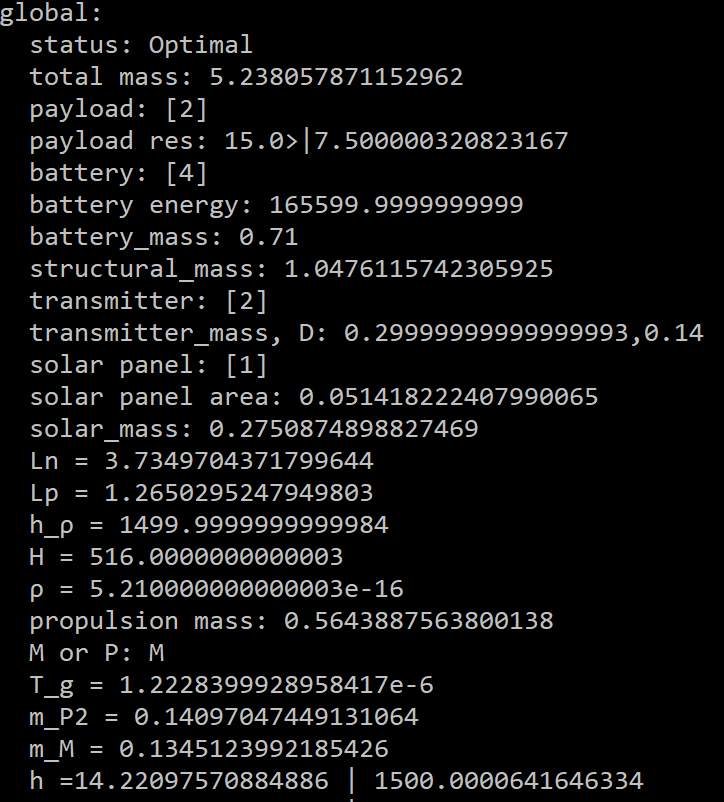
\includegraphics{https://www.dropbox.com/s/1260hniqdfjy3bh/results1.PNG?raw=1}
\caption{results1.PNG}
\end{figure}

    Payload 1 is chosen(lower aperture than payload 2, but much lighter),
and the orbit is brough to 1200km. This is the altitude that satisifies
the resolution constraint given the camera aperture. Choosing this
altitude comes at some significant propellant mass penalty, but seems to
outweight the choice of having a heavier payload with better
performance.

The optimal mass comes to \textasciitilde{}5.24kg.

    \hypertarget{m-resolution-3-years}{%
\subsubsection{2. 10m resolution, 3 years}\label{m-resolution-3-years}}

\begin{figure}
\centering
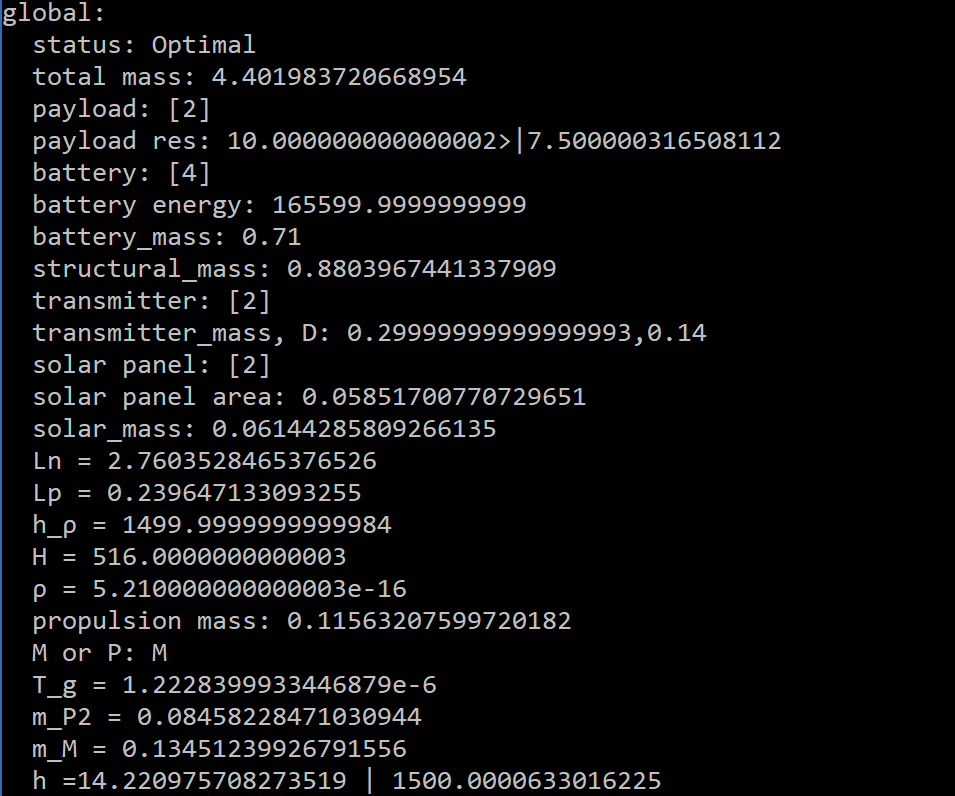
\includegraphics{https://www.dropbox.com/s/umcno6gn2a0tbkq/results2.PNG?raw=1}
\caption{results2.PNG}
\end{figure}

    This time Payload 2 is chosen(larger aperture than payload 1, but much
heavier), to meet the higher perfomance metrics required by the
resolution. This also allows the orbit to be higher (1500km), giving us
a longer lifetime and at less propellant cost.

The optimal mass comes to \textasciitilde{}4.40kg, which is lighter than
the first option.

    \hypertarget{conclusion}{%
\subsection{Conclusion}\label{conclusion}}

It took less than a minute (53s from executing the command to results),
of which 21s where spent by the backend solver(there is a significant
overhead to compile the problem, unfortunately).

This gives us the opportunity to quickly compare two different options
in a couple of minutes, versus the several weeks it might take to do it
manually.

\hypertarget{limitations-and-future-considerations}{%
\subsubsection{Limitations and future
considerations}\label{limitations-and-future-considerations}}

\begin{itemize}
\tightlist
\item
  The solver seems to sometime run into errors for no known reasons.
\item
  Further investigation should be given to how the solving time
  increases with the amount of catalog components
\item
  Make the magnetorquer and propulsion system integer variables(choices)
  from a catalog.
\end{itemize}


    % Add a bibliography block to the postdoc
    
    
    
    \end{document}
